
\documentclass[a4paper,12pt,fleqn]{article}
\usepackage{lastpage}
\usepackage{xcolor}
\usepackage{amsmath}
\usepackage{fancyhdr}
\usepackage{enumitem}
\usepackage{graphicx}
\usepackage{tabularx}
\usepackage[skip=2pt,font=small]{caption}
\usepackage{environ}
\usepackage{mdframed}
\usepackage{graphicx}


% Booleans to show answers and to ask students to return the question form
\newif\ifshowanswers

% ==============================================================================
% Question command
%
\newcounter{question}
\newcommand*\question{%
\stepcounter{question}%
\paragraph{Question \thequestion}}

% ==============================================================================
% Answer boxes
%
\mdtheorem[outerlinewidth=2,roundcorner=10pt,
leftmargin=0,rightmargin=0,
backgroundcolor=yellow!40,outerlinecolor=blue!70!black,
innertopmargin=\topskip,splittopskip=\topskip,
ntheorem=true,]{answer_box}{Answer}[section]

\NewEnviron{answer}{
\ifshowanswers
\begin{answer_box*}
\BODY
\end{answer_box*}
\fi}

% ==============================================================================
% Show answers?
%
\showanswerstrue
% \showanswersfalse


% ==============================================================================
%
% Course information
%
% ==============================================================================

\newcommand{\coursename}{Operating Systems}
\newcommand{\coursecode}{CSEx61}

\newcommand{\assigntype}{Homework Assignment \#4 \\ \textbf{Threads}}
\newcommand{\teacher}{Hatem Maohamed Ahmed (\texttt{20010447})}



% ==============================================================================
%
% Margins, header and footer
%
% ==============================================================================
\setlength{\topmargin}{0cm}
\setlength{\textheight}{9.25in}
\setlength{\oddsidemargin}{0.0in}
\setlength{\evensidemargin}{0.0in}
\setlength{\textwidth}{16cm}
\pagestyle{fancy}
\cfoot{\footnotesize{Page \thepage \ of \pageref{finalpage}
-- \coursename \ (\coursecode)}}
\renewcommand{\headrulewidth}{0pt}
\renewcommand{\footrulewidth}{0pt}

\begin{document}

% ==============================================================================
%
% Header
%
% ==============================================================================

\noindent\makebox[\linewidth]{\rule{\textwidth}{0.4pt}}

\begin{center}
\Large \textbf{\coursename} (\coursecode)
\end{center}

\begin{center}
\large \assigntype{} \\
\vspace{3mm}
\end{center}

\begin{center}
\teacher\\

\end{center}

\noindent\makebox[\linewidth]{\rule{\textwidth}{0.4pt}}


% ==============================================================================
%
% Questions
%
% ==============================================================================

% --------------------------------------------------------------------------------

% ==========================begin Question===================================
\section{Processes and Threads}

\question 
{Discuss the differences between the following:
\\a- A process and a thread in terms of the following: }
\begin{enumerate}

\item{Overhead in creation and deletion.}
\begin{answer}
{ 
- \textbf{Process}: Creating and deleting a process involves significant overhead as it requires the operating system to allocate resources such as memory space, file descriptors, and other system resources. Each process has its own address space, file descriptors, and other resources, leading to higher overhead.\\
- \textbf{Thread}: Threads are lightweight compared to processes as they share the same address space and other resources within a process. Creating and deleting threads typically have lower overhead compared to processes since threads do not require the allocation of separate resources for each thread.
}
\end{answer}

\item{Way of communication and its speed.}
\begin{answer}
{
- \textbf{Process}: Processes communicate with each other using inter-process communication  mechanisms such as pipes, message queues, shared memory, or sockets. it can be slower compared to thread communication due to the need for data copying between different address spaces.\\
- \textbf{Thread}: Threads within the same process can communicate directly through shared variables or data structures within the process's address space. Thread communication is faster than inter-process communication since threads share the same memory space and do not require data copying.
}
\end{answer}

\end{enumerate}
% ==========================end   Question===================================

% --------------------------------------------------------------------------------

% ==========================begin Question===================================
\section{TYPES OF THREADS}
\question 
{
Discuss the differences between the following: \\
a. User-level and kernel-level threads in terms of the following:
}
\begin{enumerate}

\item{
Mapping:
} 

\begin{answer}
{
- \textbf{User-level Threads}: User-level threads are totally managed by user-space libraries without kernel support.
Each user-level thread maps to a single kernel-level thread, meaning that the operating system is unaware of user-level threads and treats the entire process as a single entity. \\
- \textbf{Kernel-level Threads}: Kernel-level threads are directly supported by the operating system and each kernel-level thread maps to a separate entity in the kernel. The operating system is aware of and schedules kernel-level threads individually.
}
\end{answer}

\item
{
 Dealing with Multi-Processor Systems:
}
\begin{answer}
{
- \textbf{User-level Threads}: User-level threads are not the best for multi-processor systems because if one user-level thread in a process is blocked, all threads in that process are blocked since they share the same kernel thread. This can limit parallelism on multi-processor systems.\\
- \textbf{Kernel-level Threads}: Kernel-level threads can take advantage of multi-processor systems more effectively as each kernel thread can be scheduled independently across multiple processors, allowing for better parallelism and utilization of resources.
}
\end{answer}

\item
{
Overhead on the Kernel:
}
\begin{answer}
{
- \textbf{User-level Threads}: User-level threads have low overhead on the kernel since thread management is handled entirely in user-space libraries. Context switching between user-level threads does not involve kernel intervention, leading to lower overhead.\\
- \textbf{Kernel-level Threads}: Kernel-level threads have more overhead on the kernel as the operating system is responsible for managing and scheduling each kernel thread. Context switches between kernel threads require kernel involvement, which can lead to higher overhead compared to user-level threads.
}
\end{answer}

\item
{
Portability:
}
\begin{answer}
{
- \textbf{User-level Threads}: User-level threads are more portable across different operating systems since they are implemented using user-space libraries. The threading model can be used to the specific needs of the application without relying on specific kernel support.\\
- \textbf{Kernel-level Threads}: Kernel-level threads are less portable as they rely on operating system-specific implementations for thread management. Code using kernel-level threads may need to be modified when porting to different operating systems with different threading models.
}
\end{answer}

\item
{
Dispatching and Scheduling:
}
\begin{answer}
{
- \textbf{User-level Threads}: Dispatching and scheduling of user-level threads are handled by user-space libraries or the application itself. The operating system is not involved in thread scheduling decisions, which can lead to more flexibility but may not take advantage of system-wide optimizations.\\
- \textbf{Kernel-level Threads}: Dispatching and scheduling of kernel-level threads are managed by the operating system scheduler. The kernel determines when and on which processor a kernel thread should run, taking into account system-wide factors such as load balancing and priority scheduling.
}
\end{answer}

\end{enumerate}
% ========================== end Question====================================
% --------------------------------------------------------------------------------

% ==========================begin Question===================================

\question 
{

}
\begin{enumerate}

\item
{
Why all threads within a process will be blocked if a user-level thread calls a system call? 
}
\begin{answer}
{
	 When a user-level thread calls a system call, it blocks the entire process because user-level threads within a process share a single kernel-level thread. Since the kernel is unaware of user-level threads and manages them as a single entity, when one user-level thread makes a system call and blocks, the entire process is blocked as well. This limitation can impact the responsiveness and parallelism of the application running user-level threads, especially on multi-processor systems.
}
\end{answer}

\item{} 
{
Does that happen in kernel-level threads?
}
\begin{answer}
{
	 In kernel-level threads, each kernel-level thread is managed independently by the operating system. Therefore, if one kernel-level thread blocks due to a system call, other kernel-level threads in the same process can continue to execute without being affected. This allows for better utilization of resources and parallelism within the process.
}
\end{answer}

\end{enumerate}
% ========================== end Question====================================
% --------------------------------------------------------------------------------

% ==========================begin Question===================================

\question 
{
	List the advantages and disadvantages of user-level threads over kernel-level threads and vice versa.
}.
\begin{enumerate}

\item{} 
{
	Advantages and Disadvantages of User-level Threads:	
}.
\begin{answer}
{
\textit{\textbf{Advantages}}:\\
- \textbf{Lower overhead on the kernel}: User-level threads have minimal overhead on the kernel as thread management is handled in user-space libraries.\\
- \textbf{Portability}: User-level threads are more portable across different operating systems as they are implemented using user-space libraries.\\
- \textbf{Flexibility in scheduling}: User-level threads allow for custom scheduling algorithms tailored to the application's specific needs.\\
\textit{\textbf{Disadvantages}}:\\
- \textbf{Lack of multi-processor support}: User-level threads may not efficiently utilize multi-processor systems due to limitations in parallelism.\\
- \textbf{Blocking issues}: System calls made by user-level threads can block the entire process, limiting responsiveness.\\
- \textbf{Limited interaction with the kernel}: User-level threads may not take advantage of kernel optimizations and services.
}
\end{answer}

\item{} 
{
Advantages and Disadvantages of Kernel-level Threads:
}
\begin{answer}
{
\textit{\textbf{Advantages}}:\\
- \textbf{Multi-processor support}: Kernel-level threads can take advantage of multi-processor systems more effectively by allowing independent scheduling of each kernel thread.\\
- \textbf{Better resource utilization}: Kernel-level threads can run concurrently on different processors, improving parallelism and resource utilization.\\
- \textbf{Kernel optimizations}: Kernel-level threads can benefit from system-wide optimizations and services provided by the operating system.

\textit{\textbf{Disadvantages}}:\\
- \textbf{Higher overhead on the kernel}: Kernel-level threads incur more overhead on the kernel due to context switching and scheduling managed by the operating system.\\
- \textbf{Less portability}: Kernel-level threads are less portable across different operating systems as they rely on specific kernel implementations.\\
- \textbf{Limited flexibility in scheduling}: Kernel-level threads are subject to the operating system's scheduling policies and may not offer as much customization as user-level threads.
}
\end{answer}

\end{enumerate}
% ========================== end Question====================================
% --------------------------------------------------------------------------------

% ==========================begin Question===================================
\section{MULTICORE AND MULTITHREADING}

\question 
{
What is the faster between the process switch and the thread switch? 
}
\begin{enumerate}

\item
{
Explain why.
}
\begin{answer}
{
	thread switching is faster than process switching. This is because threads share the same address space and resources within a process, so switching between threads involves less overhead compared to switching between processes, which require a full context switch. 
	
	When switching between threads within the same process, only the thread's register values and stack need to be saved and restored, while the rest of the process's memory and resources remain intact. On the other hand, when switching between processes, the entire process context, including memory space, file descriptors, and other resources, needs to be saved and restored, leading to higher overhead.
}
\end{answer}

\end{enumerate}
% ========================== end Question====================================
% --------------------------------------------------------------------------------

% ==========================begin Question===================================

\question 
{
Would an algorithm that performs several independent calculations concurrently (for example matrix multiplication) be more efficient if it used threads or if it did not use threads? 
}
\begin{enumerate}

\item
{
	Discuss this point in both user/kernel threads and uni/multiprocessors.
}
\begin{answer}
{

- \textbf{User-level threads}: Using user-level threads for concurrent calculations can provide efficiency benefits as they have lower overhead on the kernel and can be managed within the application without involving the operating system. This allows for faster context switching between threads and better resource utilization within the process.

- \textbf{Kernel-level threads}: Kernel-level threads can also be efficient for concurrent calculations as they benefit from multi-processor support and system-wide optimizations provided by the operating system. Each kernel thread can run independently on different processors, improving parallelism and overall performance.

- \textbf{Uniprocessors}: In a uniprocessor system, using threads for concurrent calculations can still provide benefits in terms of task parallelism and resource utilization, even though true parallel execution is not possible.
  
- \textbf{Multiprocessors}: In multiprocessors system, utilizing threads for concurrent calculations can fully leverage the available processors, leading to better performance and faster computation.
}
\end{answer}

\end{enumerate}
% ========================== end Question====================================
% --------------------------------------------------------------------------------

% ==========================begin Question===================================
\section{WINDOWS PROCESS AND THREAD MANAGEMENT}
\question 
{
	Explain the states of threads in the windows operating system
}.
\begin{enumerate}

\item{} 
{
	 The states of threads in Windows include:
}
\begin{answer}
{

1. \textbf{Ready}: A thread is in the "Ready" state when it is ready to run but waiting for the processor to be allocated to it. Threads in this state are waiting in the system scheduler's queue to be selected for execution.

2. \textbf{Running}: A thread is in the "Running" state when it is actively being executed on a processor. Only one thread can be in the running state on a processor at any given time. The running thread's instructions are being executed by the processor.

3. \textbf{Waiting}: A thread is in the "Waiting" state when it is waiting for a specific event or condition to occur before it can continue execution. This could include waiting for I/O operations to complete, synchronization objects to be signaled, or timers to expire.

4. \textbf{Transition}: A thread is in the "Transition" state when it is moving between different states, such as transitioning from the "Ready" state to the "Running" state or vice versa. Threads may briefly enter this state during context switches.

5. \textbf{Standby}: A thread is in the "Standby" state when it is ready to run but waiting for its processor to become available. Threads in this state are typically associated with processors in a multi-processor system and are waiting for their assigned processor to become free.

6. \textbf{Terminated}: A thread is in the "Terminated" state when it has finished executing its code and has been terminated. Once a thread is terminated, its resources are released, and it can no longer be scheduled for execution.

}
\end{answer}

\end{enumerate}
% ========================== end Question====================================% --------------------------------------------------------------------------------

% ==========================begin Question===================================
\section{General Questions}
\question 
{
A multiprocessor with eight processors has 20 attached tape drives. There is a large number of jobs
submitted to the system that each require a maximum of four tape drives to complete execution.
Assume that each job starts running with only three tape drives for a long period before requiring
the fourth tape drive for a short period toward the end of its operation. Also assume an endless
supply of such jobs.
}
\begin{enumerate}

\item
{
Assume the scheduler in the OS will not start a job unless there are four tape drives
available. When a job is started, four drives are assigned immediately and are not released
until the job finishes. What is the maximum number of jobs that can be in progress at once?
What are the maximum and minimum number of tape drives that may be left idle as a result
of this policy?
}
\begin{answer}
{
- Maximum Number of Jobs in Progress: Since each job requires four tape drives to start, and there are only 20 tape drives available, the maximum number of jobs that can be in progress at once is 20 / 4 = 5 jobs.\\
- Maximum Number of Idle Tape Drives: In the worst-case scenario, where all 5 jobs are running and each job is using only 3 out of its 4 assigned tape drives, the total number of tape drives in use would be 5 * 3 = 15 drives. Therefore, the maximum number of idle tape drives would be 20 - 15 = 5 drives.\\
- Minimum Number of Idle Tape Drives: If all jobs are utilizing all 4 tape drives assigned to them, then there would be no idle tape drives left
}.
\end{answer}

\item
{
a- Suggest an alternative policy to improve tape drive utilization and at the same time avoid system deadlock.\\
b- What is the maximum number of jobs that can be in progress at once?\\
c- What are the bounds on the number of idling tape drives?\\
}
\begin{answer}
{
a- \textbf{Alternative Policy}: One alternative policy to improve tape drive utilization and avoid system deadlock is to allow jobs to start with fewer than four tape drives and dynamically allocate additional tape drives as needed. This dynamic allocation can be based on a priority system or a first-come-first-served basis.\\
b- \textbf{Maximum Number of Jobs in Progress}: With this alternative policy, the maximum number of jobs that can be in progress at once would depend on the total number of tape drives available and the flexibility of the allocation policy.\\
c- \textbf{Bounds on Idling Tape Drives}: The number of idling tape drives would vary based on the allocation policy. In an optimal scenario, where tape drives are efficiently allocated and utilized, the number of idling tape drives would be minimized. However, in cases where jobs are waiting for additional tape drives, there may be some idle tape drives until they are allocated.
}
\end{answer}

\end{enumerate}
% ========================== end Question====================================

% --------------------------------------------------------------------------------

% ==========================begin Question===================================

\question 
{
 Consider a multi-processor system and a multi-threaded program written using the many-to-many
threading model. Let the number of user-level threads in the program be greater than the number of
processors in the system.
Discuss the performance implications of the following scenarios:
}
\begin{enumerate}

\item
{
 The number of kernel threads allocated to the program is less than the number of processors.
}
\begin{answer}
{
 \textbf{Number of kernel threads ${<}$ Number of processors}:
 
- In this case, there are fewer kernel threads available than the number of processors. This can lead to suboptimal performance as some processors may remain idle while waiting for kernel threads to be scheduled.\\
- The system may not be able to fully utilize all available processors, resulting in potential underutilization and lower overall throughput.\\
- Context switching between user-level threads mapped to the limited kernel threads may become more frequent, leading to increased overhead and potentially degraded performance.\\
}.
\end{answer}

\item
{
 The number of kernel threads allocated to the program is equal to the number of processors.
}
\begin{answer}
{
 \textbf{Number of kernel threads = Number of processors}:
 
- When the number of kernel threads requals to the number of processors, each processor can be fully utilized by running a kernel thread. This can lead to better performance as there is no idle time for processors waiting for kernel threads.\\
- The workload can be evenly distributed across all processors, maximizing throughput and efficiency.\\
- Context switching between user-level threads mapped to kernel threads is minimized, reducing overhead and improving performance.

}
\end{answer}

\item
{
The number of kernel threads allocated to the program is greater than the number of processors
but less than the number of user-level threads.
}
\begin{answer}
{
 \textbf{Number of kernel threads ${>}$ Number of processors but ${<}$ Number of user-level threads}:
 
- In this case, there are more kernel threads available than processors, but fewer than the total number of user-level threads. This can result in a mix of scenarios a and b depending on how the kernel threads are scheduled.\\
- If the kernel scheduler efficiently assigns kernel threads to processors, performance can be improved compared to scenario a. However, there may still be some underutilization of processors.\\
- Context switching overhead may still be a concern if the kernel scheduler needs to frequently switch between user-level threads mapped to different kernel threads
}.
\end{answer}

\end{enumerate}

% ==========================begin Question===================================
\section{C Program}
\question
{
Consider the following code using POSIX threads:
}
\begin{enumerate}

\item
{
a. What does this program accomplish?\\
b. Here is the output from the executed program:\\
{.o.o.o.o.oo.o.o.o.o.o.o.o.o.o..o.o.o.o.o\\
yglobal equals 21}
Is this the output you would expect? If not, what has gone wrong?
}
\begin{answer}
	{
	a. This program creates two threads: the main thread and a separate thread created by $pthread- create$. The main thread increments the myglobal variable 20 times and prints "o" each time, while the separate thread also increments myglobal 20 times but prints "." each time. The program then waits for the separate thread to finish using $pthread-  join$ and prints the final value of myglobal.\\
	
	b. The output shown is not the output we would expect. The value of myglobal at the end should be 40 (20 increments from the main thread and 20 increments from the separate thread). However, it is only 21. This discrepancy occurs because both threads are accessing and modifying the myglobal variable concurrently without proper synchronization. This leads to a race condition where the threads can overwrite each other's changes, resulting in unexpected behavior.
	
	To fix this issue, we can use a mutex to synchronize access to the "myglobal" variable.
}
\end{answer}
	\subsection{The Given Program output}
	The following figure represents the output of the code.
	\begin{figure}[h]
	\centering
	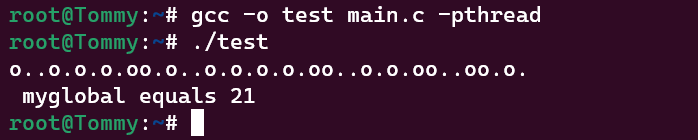
\includegraphics[width=0.9\textwidth]{output.png}
	\caption{the output from the program}
	\label{fig:terminal output}
	\end{figure}

\subsection{The Expected Program}
\subsubsection{The modifications to the program}
	The following figure represents the modifications of the code to handle the issue and to get the expected output.\\
	\begin{figure}[h]
	\centering
	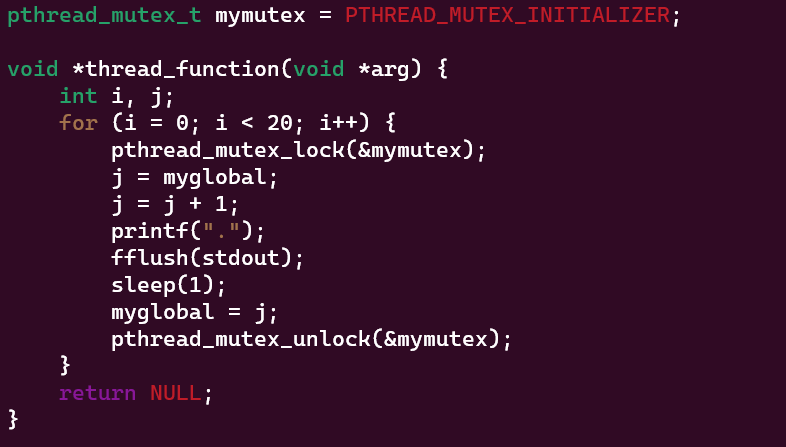
\includegraphics[width=0.9\textwidth]{output3.png}
	\caption{the modifications to the program}
	\label{fig:terminal output}
	\end{figure}\\
\subsubsection{The output of the program}
	The following figure represents the expected output of the code.
	\begin{figure}[h]
	\centering
	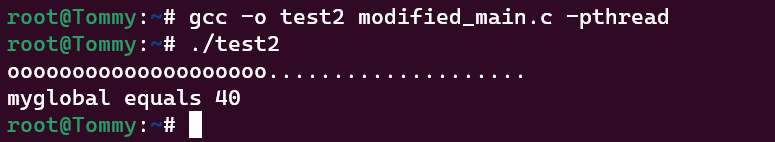
\includegraphics[width=0.9\textwidth]{output2.png}
	\caption{the output from the program}
	\label{fig:terminal output}
	\end{figure}
\end{enumerate}
% ========================== end Question====================================

\label{finalpage}
\end{document}